% !TEX root = ../main.tex
\section{Research}\label{sec:research}
% Discussion of results and evaluation
% Created an app to calibrate a ground pressure and calculate altitude from pressure data (GNSS also written up)
% Tested altitude calculation on smartphones by calibrating, travelling up Muirhead, comparing with altimeter then coming down floors.
% GPS didn't work because in building though evidence there to show poor results
% Phones matched ~altimeter altitude.
% All phones showed very similar results
% Pressure value for Galaxy different
% Altitude for one went berserk, could have been an error in the test code
We felt that it would first be a good idea to establish whether smartphones available to us can accurately calculate altitude. A testing app was created to allow us to set the reference air pressure/GNSS altitude and calculate the difference in altitude from sensor readings.
The tallest building in the University of Birmingham that we had access to at the time was Muirhead Tower, which has floors LG, G, M and 1--12. Four smartphones and a skydiving altimeter were used to test altitude detection within the building; the smartphones were the Samsung Galaxy S3, Samsung Galaxy S6, Samsung Galaxy Note 4 and the Nexus 5X.
Firstly, all devices were taken to the lowest floor (LG) and calibrated so that this would be used as the reference air pressure. Since the skydiving altimeter only activates once it sees a significant change in pressure, all devices were then taken to the top floor (12), and readings were taken from all devices. This process of taking measurements continued on every even floor down the building.
The measurements taken from the devices can be seen in Figures~\ref{fig:alt-test-altitude} and~\ref{fig:alt-test-pressure}.

\begin{figure*}[ht]
    \centering
    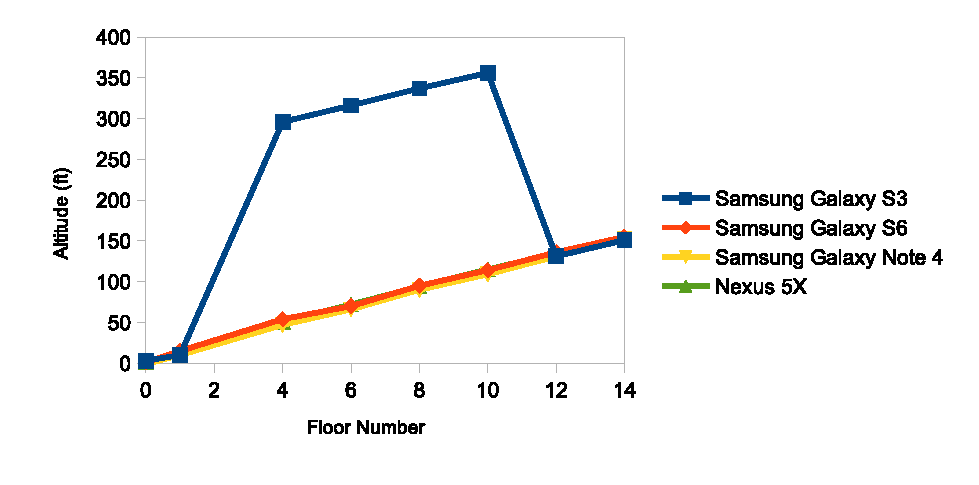
\includegraphics{alt-test-altitude}
    \caption{Altitude measurements from smartphones in Muirhead Tower}\label{fig:alt-test-altitude}
\end{figure*}

% TODO: Graph in LaTeX
% \begin{figure*}[ht]
%   \begin{tikzpicture}
%     \begin{axis}[
%       xlabel={Building Floor},
%       ylabel={Altitude (\si{\metre})},
%       xmin=0, xmax=14,
%       ymin=0, ymax=120,
%       legend pos=north west,
%       ymajorgrids=true,
%       grid style=dashed,
%       ]

%       \addplot[
%         color=blue,
%         mark=square,
%         ]
%         coordinates {
%         (0,23.1)(10,27.5)(20,32)(30,37.8)(40,44.6)(60,61.8)(80,83.8)(100,114)};
%       \legend{CuSO$_4\cdot$5H$_2$O}
%     \end{axis}
%   \end{tikzpicture}
%   \caption{Altitude measurements from Android devices while travelling up Muirhead Tower}
% \end{figure*}


\begin{figure*}[ht]
  \centering
  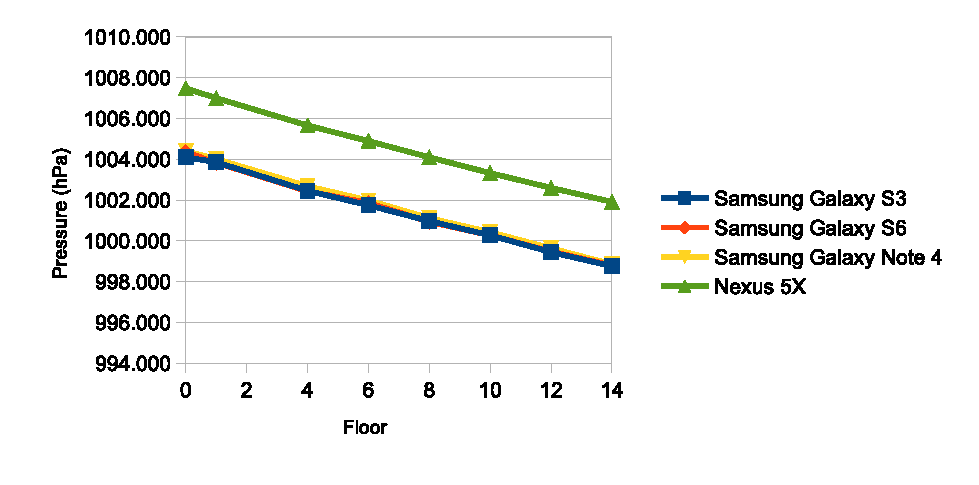
\includegraphics{alt-test-pressure}
  \caption{Air pressure measurements from smartphones in Muirhead Tower}\label{fig:alt-test-pressure}
\end{figure*}

Measurements for altitude were in feet since this is the most common unit used for skydiving in the UK and what the conventional altimeter was set to display. The skydiving altimeter that was used as a reference, unfortunately, could only be used on the top floor due to it resetting to zero if it does not detect altitude changes under a certain height. On the top floor of the building the skydiving altimeter that displays altitude in tens of feet showed a height of \SI{150}{\feet}, all smartphones showed similar readings between \SIlist{150; 160}{\feet}, as seen in Figure~\ref{fig:alt-test-altitude}.
Figure~\ref{fig:alt-test-pressure} shows that all phones follow the same rate of change in air pressure as the test moved down the floors of the building, however, the Nexus 5X appears to give higher pressure readings than the other phones. The higher pressure reading from the Nexus 5X could be due to a difference in the barometric sensor's calibration, it is likely that the Samsungs all use the same chip or similar and that the Nexus phone uses a chip from a different manufacturer.
There does seem to be some strange behaviour in the Galaxy S3's results, shown in Figure~\ref{fig:alt-test-altitude}. The altitude reading from the Galaxy S3 jumps from \SI{131}{\feet} to \SI{356}{\feet} between floors ten and eight (twelve and ten in the graph), which is not correct. Something must have changed in either the reference pressure or temperature to have caused this unexpected behaviour because when we look at results for the Galaxy S3 in Figure~\ref{fig:alt-test-pressure}, there are no strange jumps in the data. After testing again and not being able to reproduce the problem, it is entirely possible that this was due to a hard to activate bug in the test app. The test app was set up to track altitude data from GNSS as a source however many of the devices could not receive a satellite signal from within the building. The phones that could receive a GNSS signal verified previous research suggesting substantial inaccuracies in GNSS altitude data, often fluctuating by \SI{\pm10}{\feet}.

% Tested Wi-Fi Direct connection speed. Approx 4secs including time to click accept connection
Another test that has been conducted was to determine the typical time to establish a connection via Wi-Fi Direct. Three different phones were used to connect to each other across a room and timed until the word ``Connected'' showed on the screen. The time for a connection to be established across devices was approximately four seconds, including time to click ``Accept'' for the connection. Wi-Fi Direct connection times were tested to ensure that they are not too slow for the purposes we require.

% Discussion of justification for work
% Shows that smartphones may be appropriate for aiding skydivers
The altitude test has undoubtedly helped prove that today's smart devices are capable of measuring altitude to a useful degree of accuracy. Our findings were closely matched by a very similar test documented by \textcite{he_atmospheric_2012}. It is important to note that while the results are positive for demonstrating the appropriateness of using smart devices for altitude detection in some cases, this may not necessarily apply to the more extreme circumstances of skydiving.

% GNSS is inaccurate
That the GNSS data could not be used for a significant portion of the test, demonstrates why it would not be a suitable primary source for altitude data, smart devices would have to rely on having satellite signal which may not always be the case. On top of this, the altitude data provided by GNSS is inaccurate, we saw large, regular fluctuations in the altitude data produced.
